\ylDisplay{Kuup vedelikes} % Ülesande nimi
{Koit Timpmann} % Autor
{lõppvoor} % Voor
{2018} % Aasta
{P 4} % Ülesande nr.
{3} % Raskustase
{
% Teema: Mehaanika

\ifStatement
Anumas on kaks mittesegunevat vedelikku, milles heljub tahkest ainest kuup küljepikkusega $l = 10$ $cm$. Ühe vedeliku tihedus on $\rho_1 = 0,8$ $g/cm^3$, teise vedeliku tihedus $\rho_2 = 1,2$ $g/cm^3$ ja kuubi aine tihedus $\rho_k = 1,1$ $g/cm^3$ . Ülemise vedelikukihi paksus on suurem kuubi külje pikkusest. Kui sügaval alumises vedelikus asetseb kuup?
\fi


\ifHint
Ülesannet on võimalik lahendada kahte pidi. Esimesel juhul mõistame, et kehale mõjuvad kolm jõudu - raskusjõud, vedeliku rõhk ülemisele pinnale ja vedeliku rõhk alumisele pinnale. Teisel juhul mõistame, et vedelikus heljuva keha korral võrdub kehale mõjuv raskusjõud kummagi vedeliku poolt mõjuvate üleslükkejõudude summaga
\fi

\ifSolution
\begin{center}
	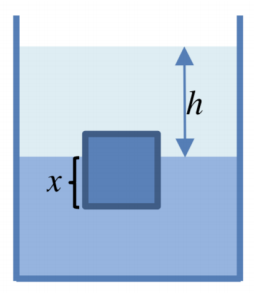
\includegraphics[width=0.5\linewidth]{2018-v3p-04-lah.PNG}
\end{center}
Lahendus 1
Kehale mõjuvad kolm jõudu - raskusjõud, vedeliku rõhk ülemisele pinnale ja vedeliku rõhk alumisele pinnale: $mg + F_1 + F_2 =0$
\begin{center}
$mg + \rho_k l^3 g$,
\end{center}
\begin{center}
$F_1 \rho_1 g (h - (l - x)) l^2$,
\end{center}
\begin{center}
$F_2 = \rho_1 g h l^2 + \rho_2 g x l^2$,
\end{center}
kus $h$ - väiksema vedelikukihi paksus, $x$ - kuubi selle osa pikkus, mis asub suurema tihedusega vedelikus. Asendame need jõud seosesse. Pärast taandamisi saame seose
\begin{center}
$(\rho_k - \rho_1)l = (\rho_2 - \rho_1)x \Rightarrow x = 7,5$ cm
\end{center}
Lahendus 2
Vedelikus hõljuva keha korral võrdub kehale mõjuv raskusjõud kummagi vedeliku poolt mõjuvate üleslükkejõudude summaga
\begin{center}
$mg = F_{y2} + F_{y1}$,
\end{center}
seega 
\begin{center}
$\rho_k l^3 g = \rho_2 g x l^2 + \rho_1 g (l - x)l^2, \Rightarrow x = \frac{ (\rho_k - \rho_1) l} {(\rho_2 - \rho_1)} = 7,5$ $cm$.
\end{center}
\fi
}
